\newcommand{\erdiagram}[1][]{E-R diagram}
\section{E-R Diagram}
In order to get an overview of how to structure the database \erdiagram[]s gives a neat foundation. The \erdiagram[] can be seen on figure \ref{fig:er_diagram}.
The \erdiagram[] is based upon the class diagram \fixme{Inds\ae{}t en reference til det f\o{}rste klasse diagram her!!}. \fixme{Kilder, kilder og en kilde.}

\begin{figure}[h]
	\centering
		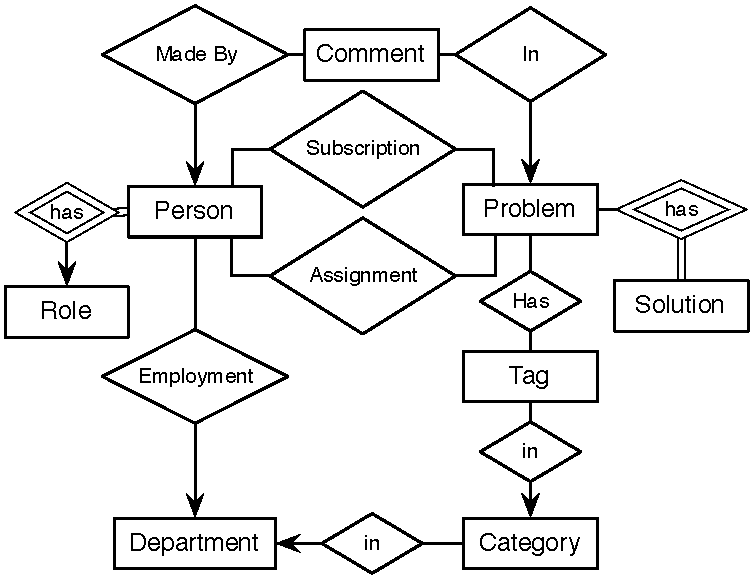
\includegraphics[scale=0.8]{input/implementation/database/ER-diagram.pdf}
	\morscaption{The ER-diagram}
	\label{fig:er_diagram}
\end{figure}

Every class is turned into a entity and every relation is turned into a relationship. The relationships contain the primary keys from the two entities it is a relation between. Only the relationship prob\_sol has an attribute beside the primary keys. This is called time and represent the time for when the solution were attach to the problem, this is used to determine when the problem is solved. The last attached solution to a solved problem must indicate the final of the solving phase. 

Any other relation does not need attributes beside the primary keys. It would only be necessary if the same entity could have more than one relation with the same entity e.g. if a system administrates a zoo, then the feeding of the tortoises could be done more than once by the same zoo keeper, and a time stamp would be necessary to avoid duplicates. In our system this problem does not occur at any point e.g. a \client[] can not be subscribed twice two the same problem. This applies to all relations. 

%a car can fill up more than once at the same gas station, 
The three classes who inherits from each other, \client[], \staff[], and \admin[] are combined into one entity named roles. This is due to that a person can only have one role, and therefore this representation is more efficient. This also gives a nice modifiability because adding a new role is simply just adding a new tuple to the entity. 
